% !TeX root = ../../Thesis.tex
\chapter{Theory}
\label{chp:theory}

Remember to refer to Notes for Cours Ecole Doctorale, Advanced Theory of Plasmas, Ecole Polytechnique Fédérale de Lausanne (Saved on Mendeley)

\section{Motivation}
\subsection{Kinetic plasma instabilities}
\subsection{Three-wave parametric instabilities}

\section{Linear theory}
The aim of the linear theory of \acrshort{SBS} is to understand how the growth
 of the instability depends on factors such as: plasma density; laser intensity; and temperature.
\subsection{Dispersion curves and linear modes}
\subsection{Zoology/topology of modes}
\subsubsection{Beam acoustic modes}
\subsubsection{Electron acoustic modes}
ie on the omega,k diagram how many things are there that we should be worried
about? BGK modes, B\cite{Kruer96}
\subsection{Landau damping}

\section{Quasi-linear theory}
%\subsection{Landau damping}

Bohm-Gross waves; Beam acoustic modes, other acoustic modes.
etc. Where are they and how do they relate? Ie the Bohm-Gross and Electron
Acoustic modes join at klD~0.53

\section{Nonlinear theory}
\subsection{Three-wave parametric instabilities}
\subsection{Nonlinear frequency shift}
\subsection{Nonlinear Landau damping}
%non-linear basis for trapping induced SRS modes found in \cite{Rose2001}, also
 %a thing called the nonlinear dielectric function

\subsection{Rosenbluth gain}

Since the instability we are concerned with is convective, we would like to understand what the maximum wave amplitude is for the daughter waves, according to the linear theory, in order to determine how SRS will grow in the fluid regime.

The derivation below follows the the steps laid out in Nishikakwa whatever 1976, with some steps written out explicitly, some changes in notation to make it easier to follow, and minor typographical corrections. 

We use our physical understanding of the system make the following assumptions:
\begin{enumerate}
	\item undamped EMW $\Gamma_1 = 0$
	\item strong damping and slow convection of EPW
	\item constant source at $-\infty$, maximum value at $+\infty$
\end{enumerate}

Consider a three-wave parametric instability that takes place in a plasma slab with a density gradient in $x$ with a uniform pump. The density gradient leads to $x$-varying wavenumbers for the waves, so we define the `wavenumber mismatch' as $\kappa = k_0(x) - k_1(x) - k_2(x)$, where perfect matching is defined by the condition $\kappa(x=0) = 0$ and we insist that $\kappa = \kappa' x$. The daughter waves can be described by the following pair of partial differential equations:

\begin{equation}
 \left(\frac{\partial}{\partial t} + v_1\frac{\partial}{\partial x} + \Gamma_1 \right)a_1 = \gamma_0a_2\text{exp}\left(i\int^x \kappa dx'\right)
\end{equation}

\begin{equation}
 \left(\frac{\partial}{\partial t} + v_2\frac{\partial}{\partial x} + \Gamma_2 \right)a_2 = \gamma_0a_1\text{exp}\left(i\int^x \kappa dx'\right);
\end{equation} 
where $\Gamma_{1,2}$ are the damping rates; $a_{1,2}$ the action amplitudes; and $v_{1,2}$ the group velocities of the two waves. 

WHAT ARE WE TRYING TO DO, WHAT MOTIVATES THIS TRANSFORM?

Recalling the definition of the Laplace transform of a function $f(t)$: $L\{f(t)\}= F(p) = \int_0^\infty e^{-pt} f(t) dt$ we take the Laplace transform of these equations to get

\begin{equation}\label{eqn:rosenbluth_laplace}
a_1(0,x) + pA_1(p,x) + \Gamma_1 A_1(p,x) + v_1\frac{\partial}{\partial x}A_1(p,x) = \gamma_0 A_2(p,x)\text{exp}\left(i\int^x \kappa dx'\right)
\end{equation}

\begin{equation}\label{eqn:rosenbluth_laplace_EPW}
a_2(0,x) + pA_2(p,x) + \Gamma_2 A_2(p,x) + v_2\frac{\partial}{\partial x}A_2(p,x) = \gamma_0 A_1(p,x)\text{exp}\left(i\int^x \kappa dx'\right).
\end{equation}

Re-writing $A_1,A_2$ to allow us to do a little trick where the exponential term on the RHS of the coupled equations disappears:  

\begin{equation}
 A_1(p,x) = \tilde{a_1}(p,x)\text{exp}\left(i\int_0^x \kappa/2 dx'\right),
\end{equation}

\begin{equation}
 A_2(p,x) = \tilde{a_2}(p,x)\text{exp}\left(-i\int_0^x \kappa/2 dx'\right),
\end{equation}

 we can re-write Equations \ref{eqn:rosenbluth_laplace} and \ref{eqn:rosenbluth_laplace_EPW} as:

\begin{equation}\label{eqn:rosenbluth_solveable_EMW}
	\left(p + \Gamma_1 + i\frac{\kappa}{2}v_1 + v_1\frac{\partial}{\partial x}\right)\tilde{a_1} = \gamma_0 \tilde{a_2} + \tilde{a_1}(0)
\end{equation}  

\begin{equation}\label{eqn:rosenbluth_solveable_EPW}
	\left(p + \Gamma_2 - i\frac{\kappa}{2}v_2 + v_2\frac{\partial}{\partial x}\right)\tilde{a_2} = \gamma_0 \tilde{a_1} + \tilde{a_2}(0)
\end{equation}  

We now consider the case where one of the two daughter waves is strongly damped and slowly convecting (in SRS this would be the EPW), in terms of the variables we have, this condition is written as $|\Gamma_2| \gg |v_2\partial / \partial x|$. We neglect the source term for $a_2$, as it is sufficient to have a source term for $a_1$ to get growth of both waves, and set p=0 (VALIDITY???). Now equation \ref{eqn:rosenbluth_solveable_EPW} allows us to write $\tilde{a_2}$ in terms of $\tilde{a_1}$ as

\begin{equation}
	\tilde{a}_2 = \frac{\gamma_0}{\Gamma_2 - i v_2 \kappa/2}\tilde{a}_1.
\end{equation} We then substitute this into Equation \ref{eqn:rosenbluth_solveable_EMW}, set the source for $\tilde{a_1}(0,0) = I\delta(x-x_0)/p$, and the damping rate for the daughter EMW to zero $(\Gamma_1=0)$, to get the following PDE describing $\tilde{a_1}$ in terms of $x$:

\begin{equation}
	\left(p + i\frac{\kappa}{2}v_1 + v_1\frac{\partial}{\partial x}\right)\tilde{a_1} = \frac{\gamma_0^2}{\Gamma_2 - i v_2 \kappa/2}\tilde{a}_1 + I\delta(x-x_0)/p
\end{equation}



\section{Autoresonance}

\begin{figure}[ht]
    \centering
    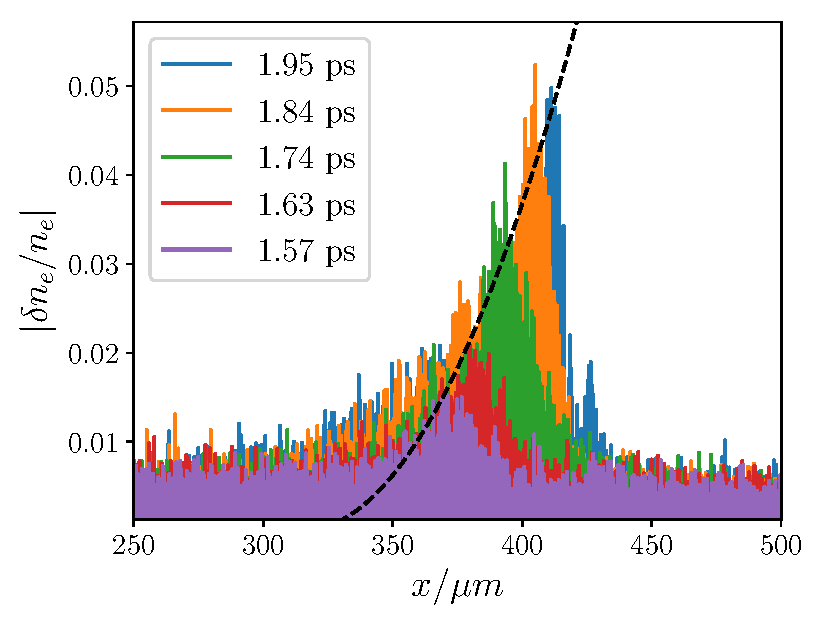
\includegraphics[width=0.8\columnwidth]{Chapters/C2_Theory/AR_diagnostic.pdf}
    \caption{Example of autoresonant growth in an EPOCH simulation with parameters: $n_{min} = 0.06 n_{\text{crit}}$; $n_{max} = 0.17 n_{\text{crit}}$; $T_e = 4.5\si{keV}$; $\text{nPPC}=10,000$; $I_0 = 2 \times 10^{15}\si{\watt / \centi\metre^2}$. Black dashed line comes from Chapman \textit{et al.} \citep{Chapman2012} formula.}
    \label{fig:AR_diagnostic}
\end{figure}{}

%\bibliographystyle{plainnat}
%\bibliography{Chapters/C2_Theory/Theory}
